\chapter{Supplemental Materials}
\label{supplementals}

To do.

% Software list/table
% DeepLabCut \href{https://github.com/DeepLabCut/DeepLabCut}
% MWorks \href{https://mworks.github.io}
% ScanImage 2016 \href{http://scanimage.vidriotechnologies.com}

% Custom software
\href{https://github.com/coxlab/behavior_rig}
\href{https://github.com/julianarhee/morph-pov}

\href{https://github.com/julianrhee/retinotopy-mapper}
\href{https://github.com/julianarhee/acquisition-tools}


% Data numbers 

\begin{table}[h]
 \caption{Data Summary}
  \centering
   \begin{tabular}{lllll}
    \toprule
    Stimulus & Area & Rats & FOVs & Cells   \\
    \midrule
    Moving bar & V1  & 5 & 12 & 1277        \\
               & LM  & 6 & 14 & 530         \\
               & LI  & 4 & 9 & 502          \\
    \midrule
    Receptive Fields & V1  & 11 & 11 & 548  \\
                     & LM  & 8 & 8 & 241   \\
                     & LI  & 10 & 10 & 279    \\
    \midrule
    Gratings & V1  & 7 & 7 & 2211     \\
             & LM  & 8 & 8 & 2084     \\
             & LI  & 7 & 7 & 966     \\
    \midrule
    Objects  & V1  & 9 & 8 & 1028   \\
             & LM  & 10 & 7 & 684   \\
             & LI  & 8 & 7 & 402    \\
    \bottomrule
  \end{tabular}
  \label{tab:data_counts}
\end{table}

% \section{Related to Chapter 1}
Aggregate training data
\begin{figure}[t!]
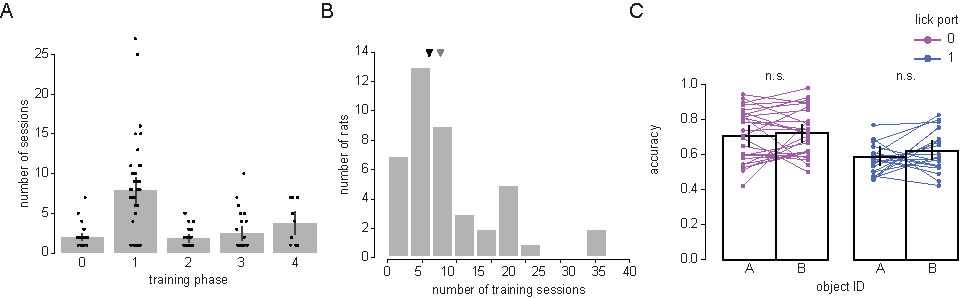
\includegraphics[width=\textwidth]{figures/supplemental/fig_s1_aggregate_training/fig_s1_aggregate_training.pdf}
    \vspace{.1in}
    \caption[Aggregate training data]{Aggregate training data. 
    \textbf{A.} Number of sessions per training phase. Each dot represents one rat. Bars show mean and SD.
    \textbf{B.} Histogram of the total number of training sessions to reach criterion (across all phases). Black and gray triangles denote the mean and median, respectively. 
    \textbf{C.} Accuracy split by object identity and port mapping. Each pair of lines represents one rat. Colors indicate object ID. 
    \label{supfig:aggregate_training}}
\end{figure}

% FIGURE S.2 MORPH
Individual performance on morphing test
\begin{figure}[t!]
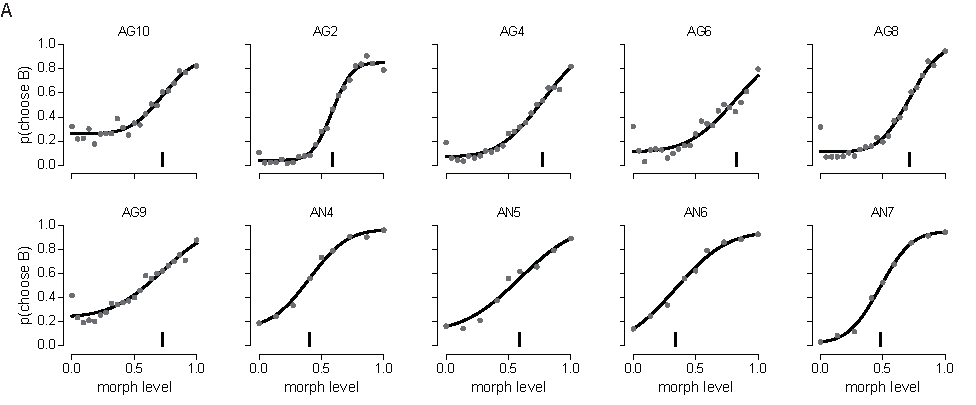
\includegraphics[width=\textwidth]{figures/supplemental/fig_s2_morphs_per_animal/fig_s2_morphs_per_animal.pdf}
    \vspace{.1in}
    \caption[Individual psychometric curves]{Individual psychometric curves for morphs. 
    \textbf{A.} 
    \label{supfig:morphs}}
\end{figure}

Individual performance on invariance test
% FIGURE S.3 INVAR
\begin{figure}[t!]
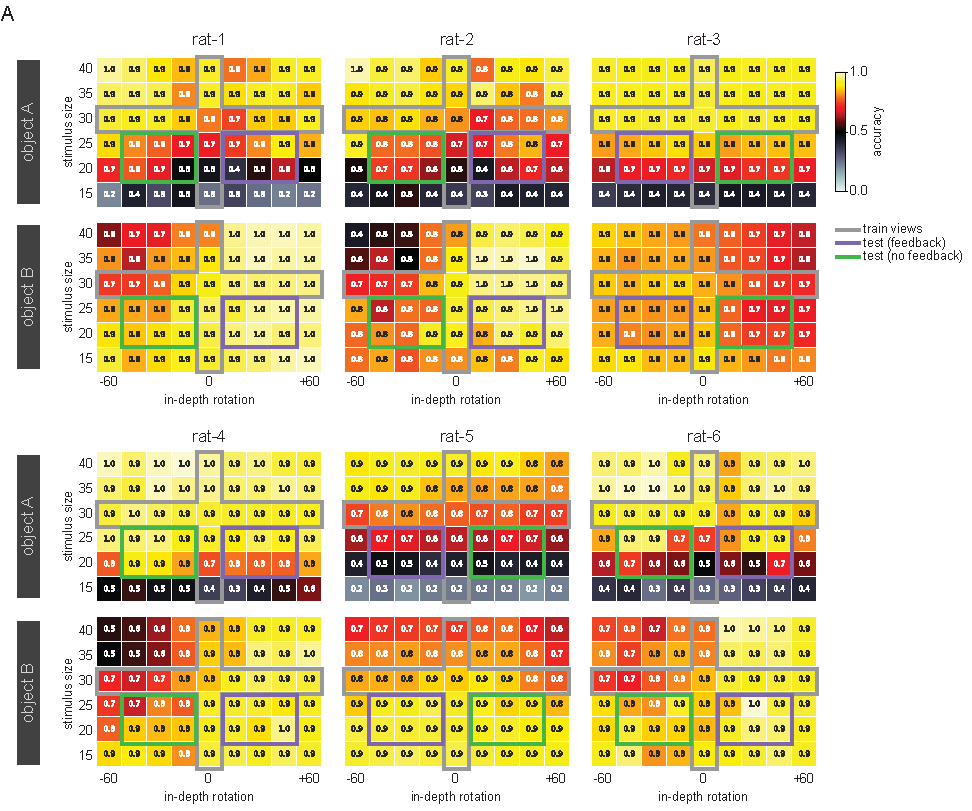
\includegraphics[width=\textwidth]{figures/supplemental/fig_s3_heatmaps_per_rat/fig_s3_heatmaps_per_rat.pdf}/
    \vspace{.1in}
    \caption[Individual invariance performance]{Individual performance on invariance test.
    \textbf{A.} 
    \label{supfig:heatmaps}}
\end{figure}

% \section{Related to Chapter 3}
% FIGURE S.4 STIMULI
\begin{figure}[t!]
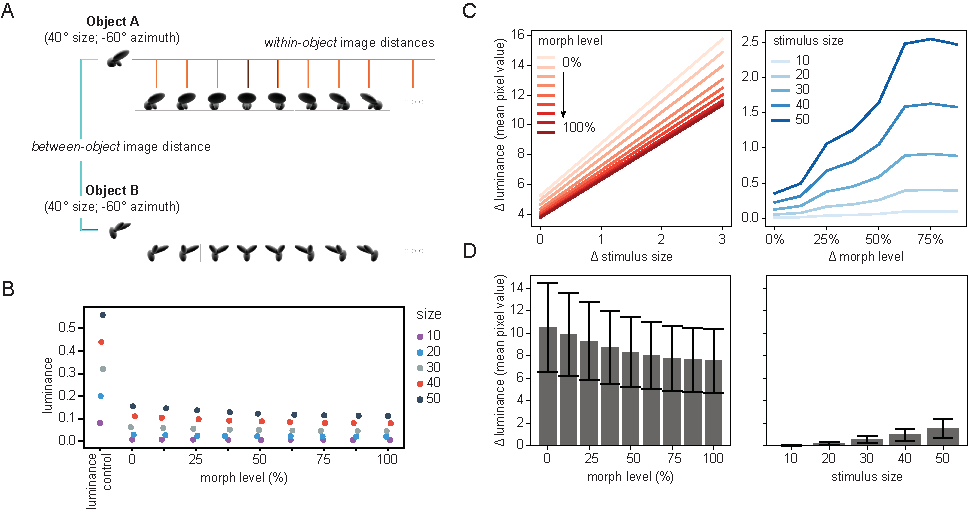
\includegraphics[width=\textwidth]{figures/supplemental/fig_s4_stimulus_metrics/fig_s4_stimulus_metrics.pdf}
    \vspace{.1in}
    \caption[Individual invariance performance]{Individual performance on invariance test.
    \textbf{A.} 
    \label{supfig:stimulus_metrics}}
\end{figure}


% \subsection{Comparison of stimulus size for receptive field measurements}

% \subsection{Demonstration of spherical correction}

% \subsection{Comparison of receptive field and gratings tuning}



% \section{Related to Chapter 4}

% \subsection{Tuning similarity as a function of distance}

% \subsection{Classifier accuracy as a function of receptive overlap}

% \subsection{Classifier generalization, matched for receptive field size}
